\section{Stolpersteine}
Bei der Berechnung der Welle mittels Potenzreihen gibt es mehrere Dinge, die 
beachtet werden m"ussen. Von besonderer Bedeutung sind die Genauigkeit der 
L"osungen f"ur die jeweiligen $x$, sowie die Zeit, welche f"ur die 
Berechnung ben"otigt wird.

\subsubsection{Genauigkeit}
Gem"ass
\begin{equation*}
	y(x) = \sum_{k=0}^{\textcolor{red}{\infty}}a_kx^k
\end{equation*}
m"usste man f"ur jedes $x$ eine unendliche Anzahl Additionen ausf"uhren, was 
bedeutet, dass die Berechnung f"ur ein einzelnes $x$ unendlich lange 
dauert. Folglich muss man die maximale Anzahl $k$ einschr"anken:
\begin{equation*}
	y(x) = \sum_{k=0}^{\textcolor{red}{k_{\text{max}}}}a_kx^k.
\end{equation*}
Das hat aber weitreichende Folgen: So werden je nach $k_{\text{max}}$ fr"uher 
oder sp"ater die L"osungswerte gegen $+\infty$ oder $-\infty$ gehen, was daran 
liegt, dass der Term $x^k$ einer endlichen Reihe gegen"uber den $a_k$ zu 
dominieren beginnen wird.

\begin{figure}
	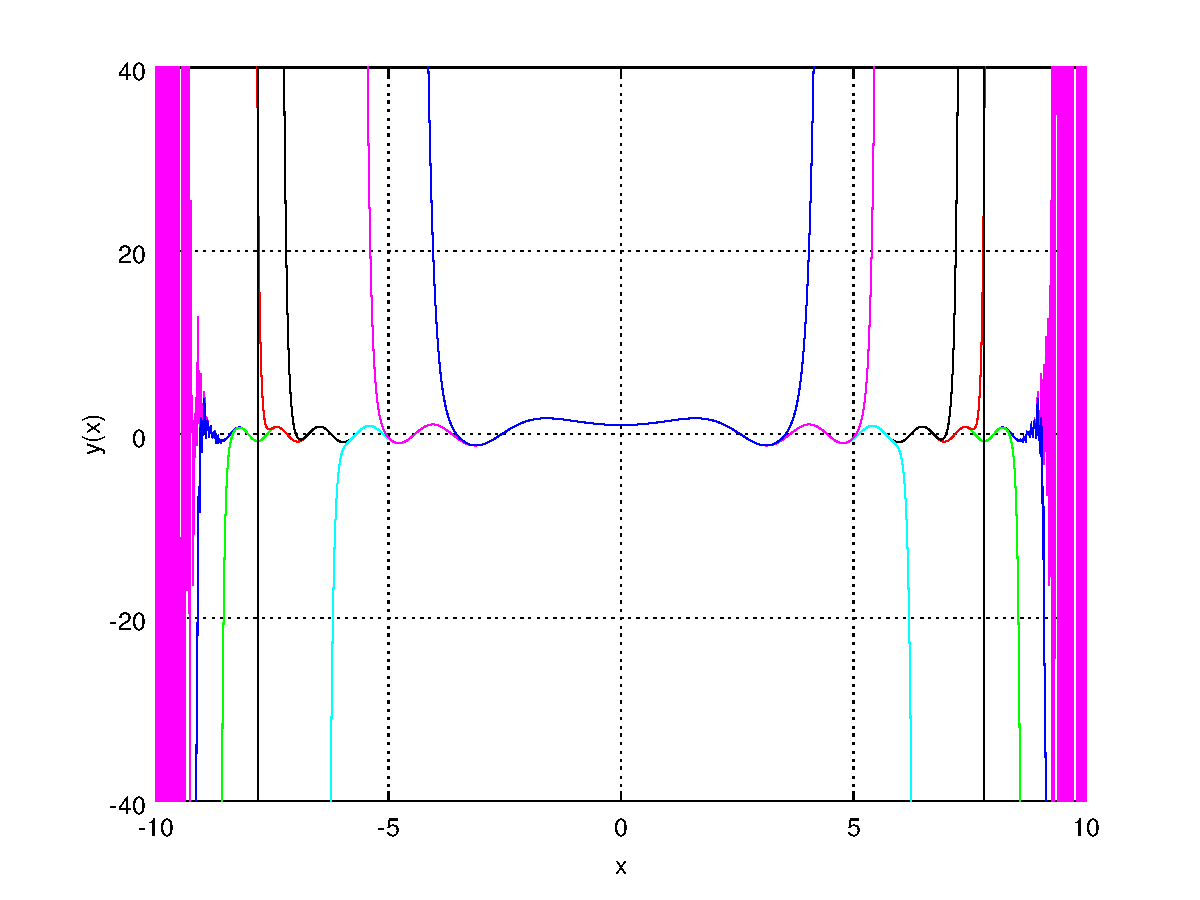
\includegraphics[width=1\hsize]{./wellen/images/kmax/kmax.pdf}
	\caption{Auswirkung $k_{\text{max}} \in [30,240]$ mit Schrittl"ange 30 auf 
	die Wellenform.}
	\label{fig:wellen:variablekmax}
\end{figure}

Die Abbildung \ref{fig:wellen:variablekmax} zeigt auf, wie sich die L"osung 
der Titelgleichung mit verschiedenen $k_{\text{max}}$ entwickelt. Es ist leicht 
zu erkennen, dass mit gr"osser werdenden $k$ auch der Punkt, an dem $x^k$ 
dominiert, sich weiter vom Entwicklungspunkt entfernt. Es taucht noch ein 
weiteres Ph"anomen auf: Da die Werte von $a_k$ immer kleiner werden und die von 
$x^k$ immer gr"osser, kommt der Rechner an seine Grenzen und beginnt 
unbrauchbare Resultate zu liefern. Diese Ungenauigkeit ist durch die bin"are 
Darstellung von Dezimalzahlen und den Limitierungen der verschiedenen 
Datentypen wie \texttt{double} oder \texttt{float} in einem Rechnersystem 
gegeben. Diese Schwierigkeiten beschr"anken sich nicht nur auf die in diesem 
Kapitel besprochenen Probleme, sondern sind inh"arent zu allen 
Berechnungsaufgaben die mit Computern ausgef"uhrt werden.

\subsubsection{Berechnungszeit}

\begin{algorithm}
	\floatname{algorithm}{Pseudocode}
	\begin{algorithmic}[1]
		\State $x \gets x_{\text{min}}$
		\For{$x \le x_{\text{max}}$}
			\State $a_{-2} \gets 0$
			\State $a_{-1} \gets 0$
			\State $a_0 \gets y(0)$
			\State $a_1 \gets y'(0)$
			\State $s_{\text{series}} \gets a_0 + a_1x$
			\State $k \gets 2$
			\For{$k \le k_{\text{max}}$}
				\State $a_k \gets -\cfrac{1}{k(k-1)}			
				(aa_{k-4}+ba_{k-3}+ca_{k-2})$
				\State $s_{\text{series}} \gets s_{\text{series}} + a_k x^k$
				\State $k \gets k + 1$
			\EndFor
			\State $x \gets x + x_{\text{step}}$
		\EndFor
	\end{algorithmic}
	\caption{Wellen Potenzreihenberechnung} 
	\label{alg:wellen:potenzreihenrechnung}
\end{algorithm}

Die Berechnung von Potenzreihenl"osungen im Intervall
$[x_{\text{min}},x_{\text{max}}]$ kann "ausserst lange dauern. Auch hier muss 
die Anzahl Berechnungen, in diesem Fall die Aufl"osung des Plots, 
eingeschr"ankt werden. Eine genauere Absch"atzung kann mit Hilfe des 
Pseudocodes \ref{alg:wellen:potenzreihenrechnung} gemacht werden. Der 
Algorithmus hat eine Laufzeit von
\begin{equation*}
	O
	\left(
		k_{\text{max}}\frac{x_{\text{max}}-x_{\text{min}}}{x_{\text{step}}}
	\right).
\end{equation*}
Da einzig vier Speicherpl"atze f"ur $a_{-2}$ bis $a_1$ ben"otigt werden, hat 
dieser Algorithmus einen Speicherverbrauch von $O(1)$.
\index{Speicheraufwand}%



\begin{algorithm}
	\floatname{algorithm}{Pseudocode}
	\begin{algorithmic}[1]
		\State $a_{-2} \gets 0$
		\State $a_{-1} \gets 0$
		\State $a_0 \gets y(0)$
		\State $a_1 \gets y'(0)$
		\State $k \gets 2$
		\For{$k \le k_{\text{max}}$}
		\State $a_k \gets -\cfrac{1}{k(k-1)} (aa_{k-4}+ba_{k-3}+ca_{k-2})$
		\State $k \gets k + 1$
		\EndFor
		\State $x \gets x_{\text{min}}$
		\For{$x \le x_{\text{max}}$}
		\State $k \gets 2$
		\State $s_{\text{pot}} \gets a_0 + a_1x$
		\For{$k \le k_{\text{max}}$}
		\State $s_{\text{pot}} \gets s_{\text{pot}} + a_k x^k$
		\State $k \gets k + 1$
		\EndFor
		\State $x \gets x + x_{\text{step}}$
		\EndFor
	\end{algorithmic}
	\caption{Wellen Potenzreihenberechnung (Alternative)}
	\label{alg:wellen:potenzreihenrechnungalt}
\end{algorithm}

Nat"urlich kann man die $a_k$ auch bereits vorg"angig berrechnen. Was uns zum 
Pseudocode \ref{alg:wellen:potenzreihenrechnungalt} f"uhrt. Dieser 
alternative Algorithmus hat eine Laufzeit von
\begin{equation*}
	\mathcal{O}
	\left(k_{\text{max}} + 
		k_{\text{max}}\frac{x_{\text{max}}-x_{\text{min}}}{x_{\text{step}}}
	\right)
	=
	\mathcal{O}
	\left(
		k_{\text{max}}
		\left(
			1+\frac{x_{\text{max}}-x_{\text{min}}}{x_{\text{step}}}
		\right)
	\right),
\end{equation*}
und einen Speicherverbrauch von
\begin{equation*}
	\mathcal{O}
	\left(
		k_{\text{max}}
	\right).
\end{equation*}